\chapter{Testing and Validation}
\label{chapter:testing-validation}

The first step to test and validate our solution was to get an article database. To have that, we filled our database with random values, so that we could check that we have configured it correctly and to have a solid base on which we could test our recommendation algorithms.
Further on, we used data from different sources, to populate our database and try our algorithms.
In the following sections we describe the sources used and the tests that we made.

\section{Data sources} 
\label{sec:testing-and-validation-data-sources}
In order to test all the functionalities of our system we needed multiple data sources, since finding a source with all the required data was not possible.
In the following section we present the data sources used. Some of them are from Adobe's previous project for publishing articles online.

\subsection{Random Database} 
\label{sec:testing-and-validation-data-sources-random-database}
This was the first data we added to our database.
In order to have data that could be used for NLP we needed to use real words. To do that, we defined a small dictionary, with a couple of hundreds of words.
The main purpose of it was to test our database for basic functionality and easily develop the system.

\subsection{Fast Company} 
\label{sec:testing-and-validation-data-sources-fast-company}
Fast Company\footnote{http://www.fastcompany.com/} is a buiness magazine that focuses on technology, buisness and design. It's online platform uses Adobe's older application and has a database, very similarly in structure to ours.
In order to get their data we made calls to their public api which returned JSON objects. Because we needed to get a large amount of data which took a lot of time, we made the api calls and processing in parallel. The api provided us with almost all the data we needed, except the rating of an article and user data. We used it for testing and improving our related algorithms.

\subsection{Movie Lens} 
\label{sec:testing-and-validation-data-sources-movie-lens}
This\footnote{http://grouplens.org/datasets/movielens/} data set was provided by GroupLens Research which collected and provided rating data sets from the MovieLens web site. We used a set of data which had  100 000 ratings from 1000 users on 1700 movies.
By using that set we were able to predict what rating would a user give to a movie, based on it's previous ratings and the ratings of other users. This data set was used for testing and improving our recommendation algorithms.

\section{Testing} 
\label{sec:testing-and-validation-testing}
In order to check that our system works accordingly to our expectations, we ran the following tests, which are described below.
We required tests both for our basic operations and our algorithms.

\subsection{Endpoints} 
\label{sec:basic-operations}
In the following sections we present some testing scenarios that validate the fact that the system's endpoints work accordingly to the use cases.

\subsubsection{Add User}
\label{sec:basic-operations-add-user}
The Add User operation is a must for our recommendation algorithm. Each user needs to have  a profile, based on which we can make article recommendations. To check that the Add User operation works we ran the following tests: 
\begin{itemize}
	\item We tried adding an user without an user id, which resulted in an error message, informing us that this endpoint requires an user id.
	\item We tried adding an user with an user id, which resulted in a HTTP 200 success message, informing us that the operation was successful.
	\item We tried adding an user with an user id and multiple data, which resulted in a HTTP 200 success message, informing us that the operation was successful.
\end{itemize}

\subsubsection{Add Article}
\label{sec:basic-operations-add-user}
The Add Article operation is a must for our recommendation algorithm. To check that the Add Article operation works we ran the following tests: 
\begin{itemize}
	\item We tried adding an article without an article id, which resulted in an error message, informing us that this endpoint requires an article id.
	\item We tried adding an article with an article id, which resulted in a HTTP 200 success message, informing us that the operation was successful.
	\item We tried adding an article with an article id and multiple data, which resulted in a HTTP 200 success message, informing us that the operation was successful.
\end{itemize}

\subsubsection{Add User Friend}
\label{sec:basic-operations-add-user}
The Add User Friend operation is required only for getting recommendations based on friends recommendations. To check that the add user friend operation works we ran the following tests: 
\begin{itemize}
	\item We tried adding an user's friend without an user id, which resulted in an error message, informing us that this endpoint requires an user id.
	\item We tried adding an user's friend without a friend id, which resulted in an error message, informing us that this endpoint requires a friend id.
	\item We tried adding an user with an user and a friend id, which resulted in a HTTP 200 success message, informing us that the operation was successful.
\end{itemize}

\subsubsection{Add User Direct Recommendation}
\label{sec:basic-operations-add-user}
The Add User Direct Recommendation, combined with Add User Friend operation provides us with the means required to make friend's based recommendations. To check that the Add User Direct Recommendation operation works we ran the following tests: 
\begin{itemize}
	\item We tried adding a friend's recommendation without an user id, which resulted in an error message, informing us that this endpoint requires an user id.
	\item We tried adding a friend's recommendation without an article id, which resulted in an error message, informing us that this endpoint requires an article id.
	\item We tried adding an user with an user and an article id, which resulted in a HTTP 200 success message, informing us that the operation was successful.
\end{itemize}

\subsubsection{Delete User}
\label{sec:basic-operations-add-user}
In order to be able to clear our database, we also need to delete users. To check that the Delete User operation works we ran the following tests: 
\begin{itemize}
	\item We tried deleting an user, without providing an user id, which resulted in an error message, informing us that this endpoint requires an user id.
	\item We tried deleting an user with an user id, which resulted in a HTTP 200 success message, informing us that the operation was successful.
\end{itemize}

\subsubsection{Update User Article History}
\label{sec:basic-operations-add-user}
In order to be able to make recommmendations based on collaborative filerting, we  needed an  user article history, which records all the articles read by the user. To check that the Update User Article History operation works we ran the following tests: 
\begin{itemize}
	\item We tried updating the article history of an user, without providing an user id, which resulted in an error message, informing us that this endpoint requires an user id.
	\item We tried updating the article history of an user, without providing an article id, which resulted in an error message, informing us that this endpoint requires an article id.
	\item We tried updating the article history of an user with an article id, which resulted in a HTTP 200 success message, informing us that the operation was successful.
\end{itemize}


\subsubsection{Get Friend's Article Recommendations}
\label{sec:basic-operations-add-user}
This endpoint allows us to get an user's article recommendations based on his friends. To check that the Get Friend's Article Recommendations operation works we ran the following tests: 
\begin{itemize}
	\item We tried getting the friend's article recommendation of an user, without providing an user id, which resulted in an error message, informing us that this endpoint requires an user id.
	\item We tried getting the friend's article recommendation of an user with an article id, which resulted in a HTTP 200 success message, informing us that the operation was successful.
	\item We checked that we are getting the correct answer by adding a friend and a friend's recommended article and that we are getting the added article.
\end{itemize}

\subsubsection{Get Articles}
\label{sec:basic-operations-add-user}
This endpoint allows us to get a certain number of articles from the database. To check that the Get Friend's Article Recommendations operation works we ran the following tests: 
\begin{itemize}
	\item We added a couple of articles, by using the Add Article operation, after which we checked if the Get Articles operation returns the added articles.
\end{itemize}


\subsubsection{Get Recommended Articles}
\label{sec:basic-operations-add-user}
This endpoint allows us to get the recommended articles for an user, based on his history. To check that the Get Recommended Articles operation works we ran the following tests: 
\begin{itemize}
	\item We tried getting the recommended articles, without providing an user id, which resulted in an error message, informing us that this endpoint requires an user id.
	\item We tried getting the recommended articles of an user with an user id, which resulted in a list of articles recommended for that user in JSON format.
\end{itemize}

\subsubsection{Get Related Articles}
\label{sec:basic-operations-add-user}
This endpoint allows us to get the articles related to another article, based on it's attributes. To check that the Get Related Articles operation works we ran the following tests: 
\begin{itemize}
	\item We tried getting the related articles, without providing an article id, which resulted in an error message, informing us that this endpoint requires an article id.
	\item We tried getting the recommended articles with an article id, which resulted in a list of articles related to that article, in JSON format.
\end{itemize}

\subsubsection{Get Articles Related to a Collection}
\label{sec:basic-operations-add-user}
This endpoint allows us to get the articles related to a collection, based on it's attributes and the attributes of the articles in the collection. To check that the Get Articles Related to a Collection operation works we ran the following tests: 
\begin{itemize}
	\item We tried getting the articles related to a collection, without providing any of the collection's attributes, which resulted in an error message, informing us that this endpoint requires the collection's attributes, which are simillar to that of an article.
	\item We tried getting the related articles with a collection's attributes, which resulted in a list of articles related to that collection, in JSON format.
	\item We tried getting the related articles with a collection's attributes and a list of articles ids which are in that collection, which resulted in a list of articles related to that collection, in JSON format.
\end{itemize}

\section{Evaluation} 
\label{sec:evaluation}
In this section we describe how we evaluated our system and how well it performs.
We can apply three types of experiments, in order to evaluate our recommender's quality \cite{evaluate-recommender-system}. The first one is an offline setting, where recommendations are compared without user interaction. The second one is based on user studies, where a group of subjects interact with the system and report on the experience. The third one and the best is represented by large a scale, online experiment, where we test the system in a production environment.

\subsection{Time and Memory Usage}
\label{sec:time-memory-usage}
In the following subsections we make an analysis of the time and memory usage of our system, when applying the related and recommended algorithms, compared to solr. 

\subsubsection{Article Indexing Time}
\label{sec:article-indexing-time}

\begin{figure}[h]
\centering
\caption{Article Indexing Time}
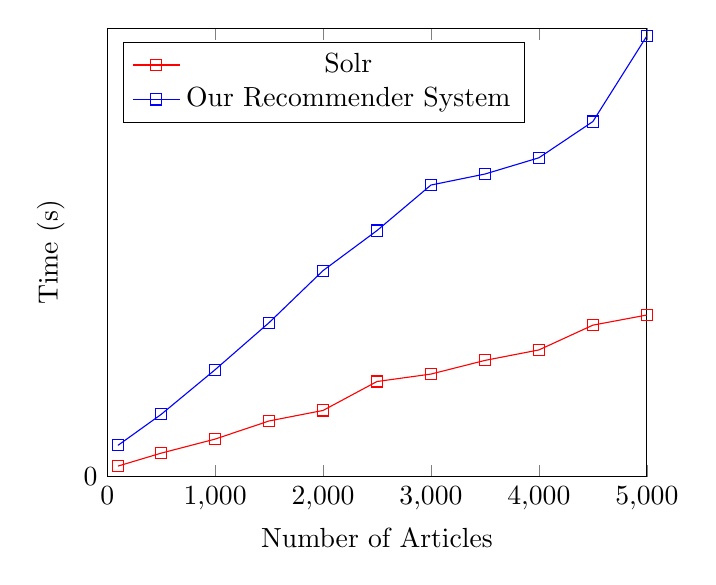
\begin{tikzpicture}
\begin{axis}[
    xlabel={Number of Articles},
    ylabel={Time (s)},
    xmin=0, xmax=5000,
    ymin=0, ymax=42,
    xtick={0, 1000,2000, 3000, 4000, 5000},
    ytick={0,50,100,150,200,250},
    legend pos=north west,
    ymajorgrids=true,
    grid style=dashed,
]
\addplot[
    color=red,
    mark=square,
    ]
    coordinates {
    (100,0.980)(500,2.192)(1000,3.509)(1500,5.208)(2000,6.192)(2500,8.903)(3000,9.600)(3500,10.880)(4000,11.862)(4500,14.183)(5000,15.132)
    };
 
 \addplot[
    color=blue,
    mark=square,
    ]
    coordinates {
    (100,2.921)(500,5.823)(1000,10.009)(1500,14.418)(2000,19.292)(2500,23.045)(3000,27.309)(3500,28.340)(4000,29.862)(4500,33.256)(5000,41.269)
    };
    \legend{Solr,Our Recommender System}
\end{axis}
\end{tikzpicture}
\label{tikz}
\end{figure}

Indexing time refers to the amount of time needed by a system to add a new item or a group of items to it's data. We have to index items in order to make the system aware of the existing information and to make certain optimisations that lower our response time.
In the above image, Figure 5.1, we can see our and solr's performance on item indexing. Our time is slower than that of solr because we use a database to store our data. This allows us to keep it in a structured manner and provide personalised recommendations, a feature that solr does not have.

\subsubsection{Related Article Time}
\label{sec:related-articles-time}

\begin{figure}[h]
\centering
\caption{Related Article Time}

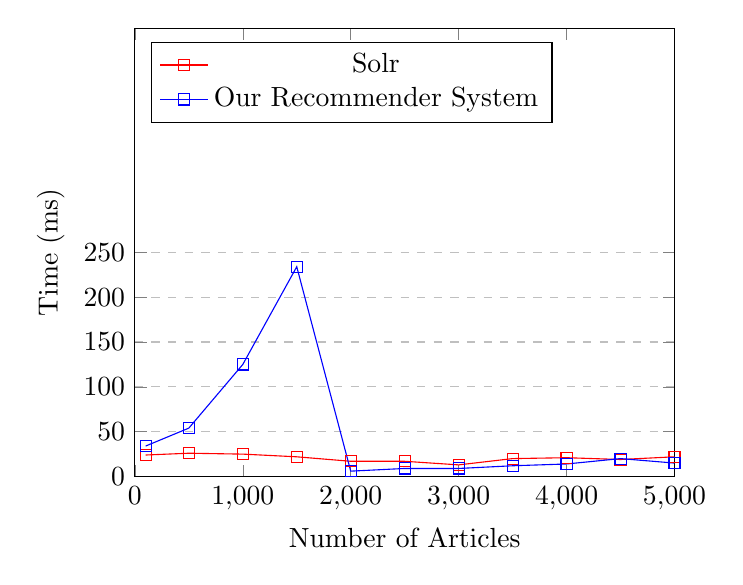
\begin{tikzpicture}
\begin{axis}[
    xlabel={Number of Articles},
    ylabel={Time (ms)},
    xmin=0, xmax=5000,
    ymin=0, ymax=500,
    xtick={0, 1000,2000, 3000, 4000, 5000},
    ytick={0,50,100,150,200,250},
    legend pos=north west,
    ymajorgrids=true,
    grid style=dashed,
]
\addplot[
    color=red,
    mark=square,
    ]
    coordinates {
    (100,24)(500,26)(1000,25)(1500,22)(2000,17)(2500,17)(3000,13)(3500,20)(4000,21)(4500,19)(5000,22)
    };
 
 \addplot[
    color=blue,
    mark=square,
    ]
    coordinates {
    (100,34)(500,54)(1000,125)(1500,234)(2000,6)(2500,9)(3000,9)(3500,12)(4000,14)(4500,20)(5000,15)
    };
    \legend{Solr,Our Recommender System}
\end{axis}
\end{tikzpicture}
\label{tikz}
\end{figure}

In Figure 5.2, we can see how solr's and our related article recommendations perform. In the begining of the experiment we didn't use any form of caching, thus using less RAM memory but we got a response time that is worse than that of solr. Then, we started using our caching mechanisms and we got a simillar time.
\subsubsection{Disk Memory Usage}
\label{sec:disk-memory-usage}

\begin{figure}[h]
\centering
\caption{Disk Memory Usage}

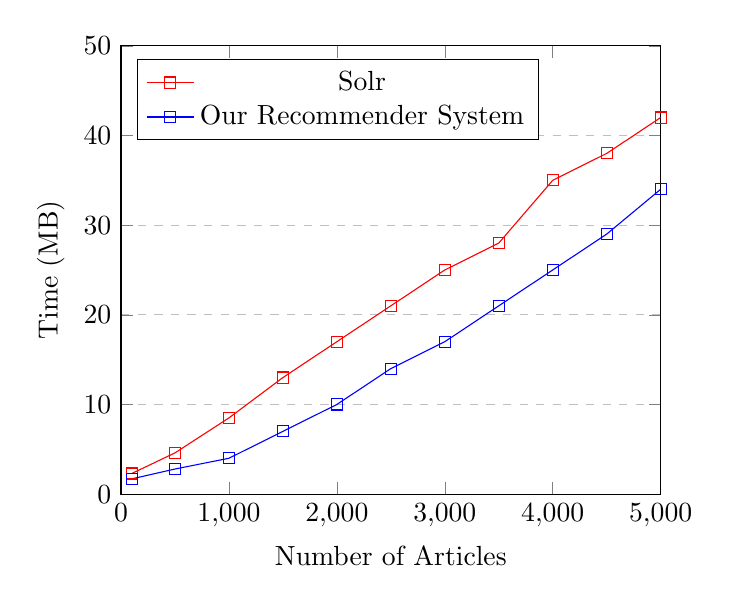
\begin{tikzpicture}
\begin{axis}[
    xlabel={Number of Articles},
    ylabel={Time (MB)},
    xmin=0, xmax=5000,
    ymin=0, ymax=50,
    xtick={0, 1000,2000, 3000, 4000, 5000},
    ytick={0,10,20,30,40,50},
    legend pos=north west,
    ymajorgrids=true,
    grid style=dashed,
]
\addplot[
    color=red,
    mark=square,
    ]
    coordinates {
    (100,2.3)(500,4.6)(1000,8.5)(1500,13)(2000,17)(2500,21)(3000,25)(3500,28)(4000,35)(4500,38)(5000,42)
    };
 
 \addplot[
    color=blue,
    mark=square,
    ]
    coordinates {
    (100,1.7)(500,2.8)(1000,4)(1500,7)(2000,10)(2500,14)(3000,17)(3500,21)(4000,25)(4500,29)(5000,34)
    };
    \legend{Solr,Our Recommender System}
\end{axis}
\end{tikzpicture}
\label{tikz}
\end{figure}

In the above image, Figure 5.3, we can see how solr's disk usage compares to ours. We can clearly see that we use less memory than solr. Even though, this may cause some speed issues, when using it without caching, our system is ideal for applications that have a limited amount of memory at their disposal.
\subsection{Quality of Results}
\label{sec:quality-of-results}
In the following subsections we make an analysis of the results quality given by our system, when applying the related or recommended algorithms.

\subsubsection{Related Articles}
\label{sec:related-articles}
Because it was almost impossible to check if we got good and relevant results with a random database we had to take a database from a previous project of Adobe, which was used by one of their clients, Fast Company\footnote{http://www.fastcompany.com/}. 

After we populated our database with their data, we started running tests on it by changing the importance of each attribute and printing the top 100 results

In order to check that we were obtaining  good results we chose an article and google searched it's title on fast company’s site. We then classified the outputs in 3 categories, by relevance, and saved the data in an expected file.

Using the expected data we then binary searched for the best importance of each attribute.
Because the expected data that we chose may have been influenced by subjective factors, we decided to test our recommendation system by using solr.

Using the best importance values we determined by using the expected file, we got our ten most related articles in solr's top 25 related.

In order to further confirm that our resulted articles are really related I built a simple web page in which users chose one of 4 degrees of relatedness and the data was saved on a server.

\subsubsection{Recommended Articles}
\label{sec:recommended-articles}
In order to test that the system gives good recommendations we took the dataset of MovieLens which provided 100,000 ratings from 1000 users on 1700 movies. Using that data we then used our algorithms to predict what rating would a user give to a certain movie, already rated, and compared it to the actual given rating. By doing this we obtained a deviation from the removed rating of about 15\%.